% !TEX root = presentation.tex
\section{Approach}
\subsection{Process}
\frame{\frametitle{Process}
  \begin{enumerate}
    \item Collect mutation score data of the software system under test.
    \item Collect source code metric data of the software system under test.
    \item Collect test suite metrics data of the software system under test.
    \item Synthesis collected data together and store it within a database.
    \item Construct classification model.
    \item Predict with classification model.
  \end{enumerate}
}

\subsection{Data Collection}
\frame{\frametitle{Data Collection}
  \begin{columns}
  	\begin{column}{5.75cm}
    	\flushleft
      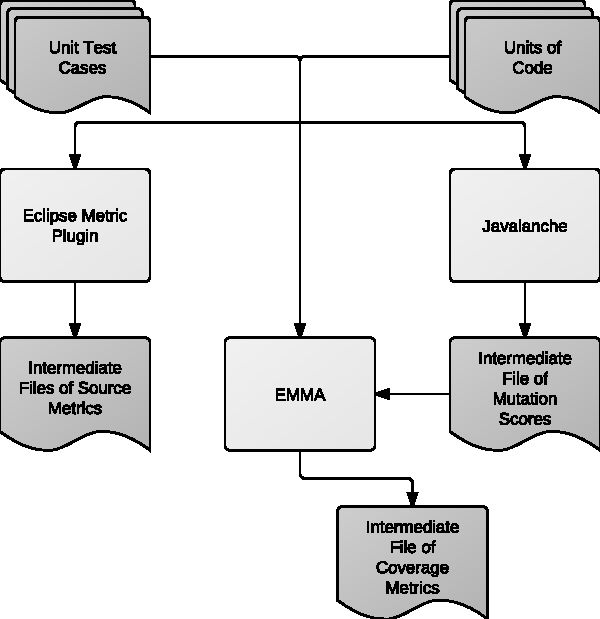
\includegraphics[width=5.25cm]{../thesis/figures/process_a_clean.pdf}
      \vspace{-4mm}
      \Huge \centering
      \ldots
    \end{column}
    \qquad
    \begin{column}{5.75cm}
      \begin{itemize}
        \item Input -- Units of test cases and units of source code:
        \begin{enumerate}
          \item Collect mutation scores using \textit{Javalanche}\footnote{\tiny{\url{github.com/david-schuler/javalanche}}}.
          \item Collect source code metrics using \textit{Eclipse Metrics Plugin}\footnote{\tiny{\url{metrics2.sourceforge.net/}}}.
          \item Collect coverage metrics using \textit{EMMA}\footnote{\tiny{\url{emma.sourceforge.net/}}}.
        \end{enumerate}
      \end{itemize}
    \end{column}
  \end{columns}
}

\subsection{Data Synthesis}
\frame{\frametitle{Data Synthesis}
  \begin{columns}
  	\begin{column}{5.75cm}
      \Huge \centering
      \ldots
      \vspace{-2mm}
      \flushleft
      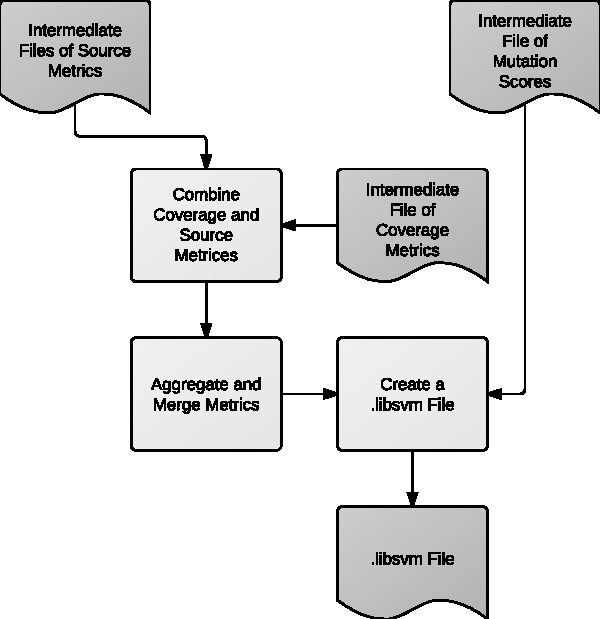
\includegraphics[width=5.25cm]{../thesis/figures/process_b_clean.pdf}
    \end{column}
    \qquad
    \begin{column}{5.75cm}
      \begin{itemize}
        \item Goal -- Category/feature data for source code units:
        \begin{enumerate}
          \item Combine source code and coverage metrics together.
          \item Merge source code metrics of the touched tests for each source code unit.
          \item Aggregate method-level source code unit metrics into class-level source code units.
          \item Create \texttt{.libsvm} file using feature/category data.
        \end{enumerate}
      \end{itemize}
    \end{column}
  \end{columns}
}

\subsection{Prediction}
\frame{\frametitle{Prediction}
  \begin{columns}
  	\begin{column}{4.75cm}
      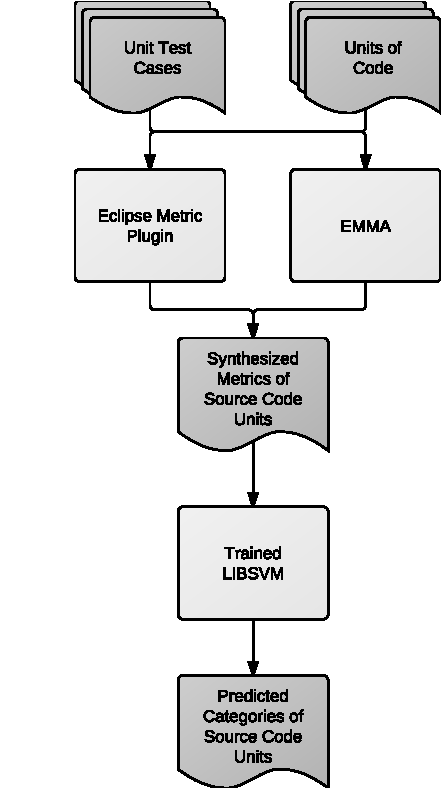
\includegraphics[width=4cm]{../thesis/figures/process_prediction_clean.pdf}
    \end{column}
    \qquad
    \begin{column}{6.75cm}
      \begin{enumerate}
        \item Collect source code and test suite metrics.
        \item Synthesis collected metrics.
        \item Use trained LIBSVM\footnote{\tiny{\url{csie.ntu.edu.tw/~cjlin/libsvm/}}} to make prediction for source code units.
      \end{enumerate}
    \end{column}
  \end{columns}
}

\subsection{Related Work}
\frame{\frametitle{Related Work}
  \begin{itemize}
  	\item Fault localization:
		\begin{itemize}
		  \item Using source code~\footcite{MKPS00}.
		  \item Using bug reports~\footcite{KL05}.
		  \item Using test coverage~\footcite{WDC10}.
		\end{itemize}
		\item Relationship between test effectiveness, test coverage and test suite size~\footcite{Ino12}.
  \end{itemize}
}
